% Prepared estimation/design mechanism; one shared source for print and web.
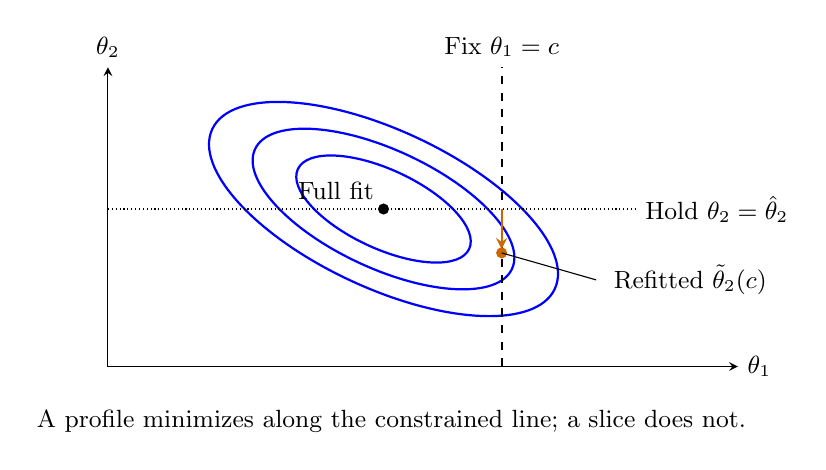
\begin{tikzpicture}[>=stealth,every node/.style={font=\small}]
\draw[->] (0,0)--(8,0) node[right]{$\theta_1$};\draw[->] (0,0)--(0,3.8) node[above]{$\theta_2$};
\foreach \a/\b in {1.2/.5,1.8/.75,2.4/1}{\draw[blue,thick,rotate around={-25:(3.5,2)}] (3.5,2) ellipse[x radius=\a cm,y radius=\b cm];}
\draw[thick,dashed] (5,0)--(5,3.8) node[above] {Fix $\theta_1=c$};
\draw[densely dotted] (0,2)--(6.7,2) node[right] {Hold $\theta_2=\hat\theta_2$};
\fill (3.5,2) circle(2pt) node[above left] {Full fit};
\fill[orange!80!black] (5,1.44299983) circle(2pt);
\draw[thin] (5,1.44299728)--(6.2,1.1);
\node[anchor=west] at (6.3,1.1) {Refitted $\tilde\theta_2(c)$};
\draw[->,thick,orange!80!black] (5,2)--(5,1.49);
\node at (3.6,-.7) {A profile minimizes along the constrained line; a slice does not.};
\end{tikzpicture}
